\documentclass[english,nohyper,titlepage]{tufte-handout}\usepackage{graphicx, color}
%% maxwidth is the original width if it is less than linewidth
%% otherwise use linewidth (to make sure the graphics do not exceed the margin)
\makeatletter
\def\maxwidth{ %
  \ifdim\Gin@nat@width>\linewidth
    \linewidth
  \else
    \Gin@nat@width
  \fi
}
\makeatother

\definecolor{fgcolor}{rgb}{0.2, 0.2, 0.2}
\newcommand{\hlnumber}[1]{\textcolor[rgb]{0,0,0}{#1}}%
\newcommand{\hlfunctioncall}[1]{\textcolor[rgb]{0.501960784313725,0,0.329411764705882}{\textbf{#1}}}%
\newcommand{\hlstring}[1]{\textcolor[rgb]{0.6,0.6,1}{#1}}%
\newcommand{\hlkeyword}[1]{\textcolor[rgb]{0,0,0}{\textbf{#1}}}%
\newcommand{\hlargument}[1]{\textcolor[rgb]{0.690196078431373,0.250980392156863,0.0196078431372549}{#1}}%
\newcommand{\hlcomment}[1]{\textcolor[rgb]{0.180392156862745,0.6,0.341176470588235}{#1}}%
\newcommand{\hlroxygencomment}[1]{\textcolor[rgb]{0.43921568627451,0.47843137254902,0.701960784313725}{#1}}%
\newcommand{\hlformalargs}[1]{\textcolor[rgb]{0.690196078431373,0.250980392156863,0.0196078431372549}{#1}}%
\newcommand{\hleqformalargs}[1]{\textcolor[rgb]{0.690196078431373,0.250980392156863,0.0196078431372549}{#1}}%
\newcommand{\hlassignement}[1]{\textcolor[rgb]{0,0,0}{\textbf{#1}}}%
\newcommand{\hlpackage}[1]{\textcolor[rgb]{0.588235294117647,0.709803921568627,0.145098039215686}{#1}}%
\newcommand{\hlslot}[1]{\textit{#1}}%
\newcommand{\hlsymbol}[1]{\textcolor[rgb]{0,0,0}{#1}}%
\newcommand{\hlprompt}[1]{\textcolor[rgb]{0.2,0.2,0.2}{#1}}%

\usepackage{framed}
\makeatletter
\newenvironment{kframe}{%
 \def\at@end@of@kframe{}%
 \ifinner\ifhmode%
  \def\at@end@of@kframe{\end{minipage}}%
  \begin{minipage}{\columnwidth}%
 \fi\fi%
 \def\FrameCommand##1{\hskip\@totalleftmargin \hskip-\fboxsep
 \colorbox{shadecolor}{##1}\hskip-\fboxsep
     % There is no \\@totalrightmargin, so:
     \hskip-\linewidth \hskip-\@totalleftmargin \hskip\columnwidth}%
 \MakeFramed {\advance\hsize-\width
   \@totalleftmargin\z@ \linewidth\hsize
   \@setminipage}}%
 {\par\unskip\endMakeFramed%
 \at@end@of@kframe}
\makeatother

\definecolor{shadecolor}{rgb}{.97, .97, .97}
\definecolor{messagecolor}{rgb}{0, 0, 0}
\definecolor{warningcolor}{rgb}{1, 0, 1}
\definecolor{errorcolor}{rgb}{1, 0, 0}
\newenvironment{knitrout}{}{} % an empty environment to be redefined in TeX

\usepackage{alltt}
\usepackage{charter}
\usepackage{helvet}
\renewcommand{\familydefault}{\rmdefault}
\usepackage[latin9]{inputenc}
\usepackage{color}
\usepackage{natbib}
\usepackage{babel}
\usepackage{graphicx}
\usepackage{amsmath}
\usepackage[unicode=true,pdfusetitle,bookmarks=true,bookmarksnumbered=false,bookmarksopen=false,
            breaklinks=false,pdfborder={0 0 0},backref=false,colorlinks=true] {hyperref}
\hypersetup{urlcolor= RedOrange, citecolor=RedOrange, linkcolor=RedOrange}
\fancyhf{}% clear previous contents of running heads/feet
\fancyhead[RE]{\footnotesize{Comparing Correlation Measures\qquad{} \thepage}}
\fancyhead[LO]{\footnotesize{\thepage \qquad{}Comparing Correlation Measures}}
\makeatletter


\title{\huge{A Comparison of \\\noindent Correlation Measures}}
\author{{\small Michael Clark\\
         \noindent Center for Social Research\\
         \noindent University of Notre Dame\\}}
%% Because html converters don't know tabularnewline
\providecommand{\tabularnewline}{\\}


\AtBeginDocument{
\def\labelitemi{} %%%%\(\cdot\) remove bullet
}

\makeatother
\IfFileExists{upquote.sty}{\usepackage{upquote}}{}

\begin{document}
\bibliographystyle{apa}

\maketitle
\pagebreak{}
\tableofcontents{}

\pagebreak{}

%%%%%%%%%%%%%%%%%%
\part{Preface} %%%
%%%%%%%%%%%%%%%%%%
This document provides a brief comparison of the ubiquitous Pearson product-moment correlation coefficient with other approaches measuring dependencies among variables, and attempts to summarize some recent articles regarding the newer measures.  No particular statistical background is assumed besides a basic understanding of correlation.  To view graphs as they are intended to be seen, make sure that the 'enhance thin lines' option is unchecked in your Acrobat Reader preferences, or just use another pdf reader.
\marginnote{Current version date \today{}.  Original April 2013. I will likely be coming back to this for further investigation and may make notable changes at that time.}
\pagebreak{}


%%%%%%%%%%%%%%%%%%%%%%%
\part{Introduction} %%%
%%%%%%%%%%%%%%%%%%%%%%%
The Pearson correlation coefficient has been the workhorse for understanding bivariate relationships for over a century of statistical practice.  It's easy calculation and interpretability means it is the go to measure of association in the overwhelming majority of applied practice.

Unfortunately, the Pearson $r$ is not a useful measure of dependency \emph{in general}.  Not only does correlation not guarantee a causal relationship as Joe Blow on the street is quick to remind you, a lack of correlation does not even mean there is no relationship between two variables.  For one, it is best suited to continuous, normally distributed data\sidenote{Not that that stops people from using it for other things.}, and is easily swayed by extreme values. It is also a measure of \emph{linear} dependency, and so will misrepresent any relationship that isn't linear, which occurs very often in practice.

Here we will examine how the Pearson $r$ compares to other measures we might use for both linear and nonlinear relationships.  In particular we will look at two measures \emph{distance correlation} and the \emph{maximal information coefficient}.

%%%%%%%%%%%%%%%%%%%%%%%%%%%%%
\section{Pearson Correlation}
As a reminder, the sample Pearson $r$ is calculated as follows: \\

\medskip
$cov_{xy} = \overset{N}{\underset{i=1}{\sum}}\frac{(x_i-\bar{X})(y_i-\bar{Y})}{N-1}$

\medskip
$r_{xy} = \frac{cov_{xy}}{var_xvar_y}$
\medskip

\marginnote{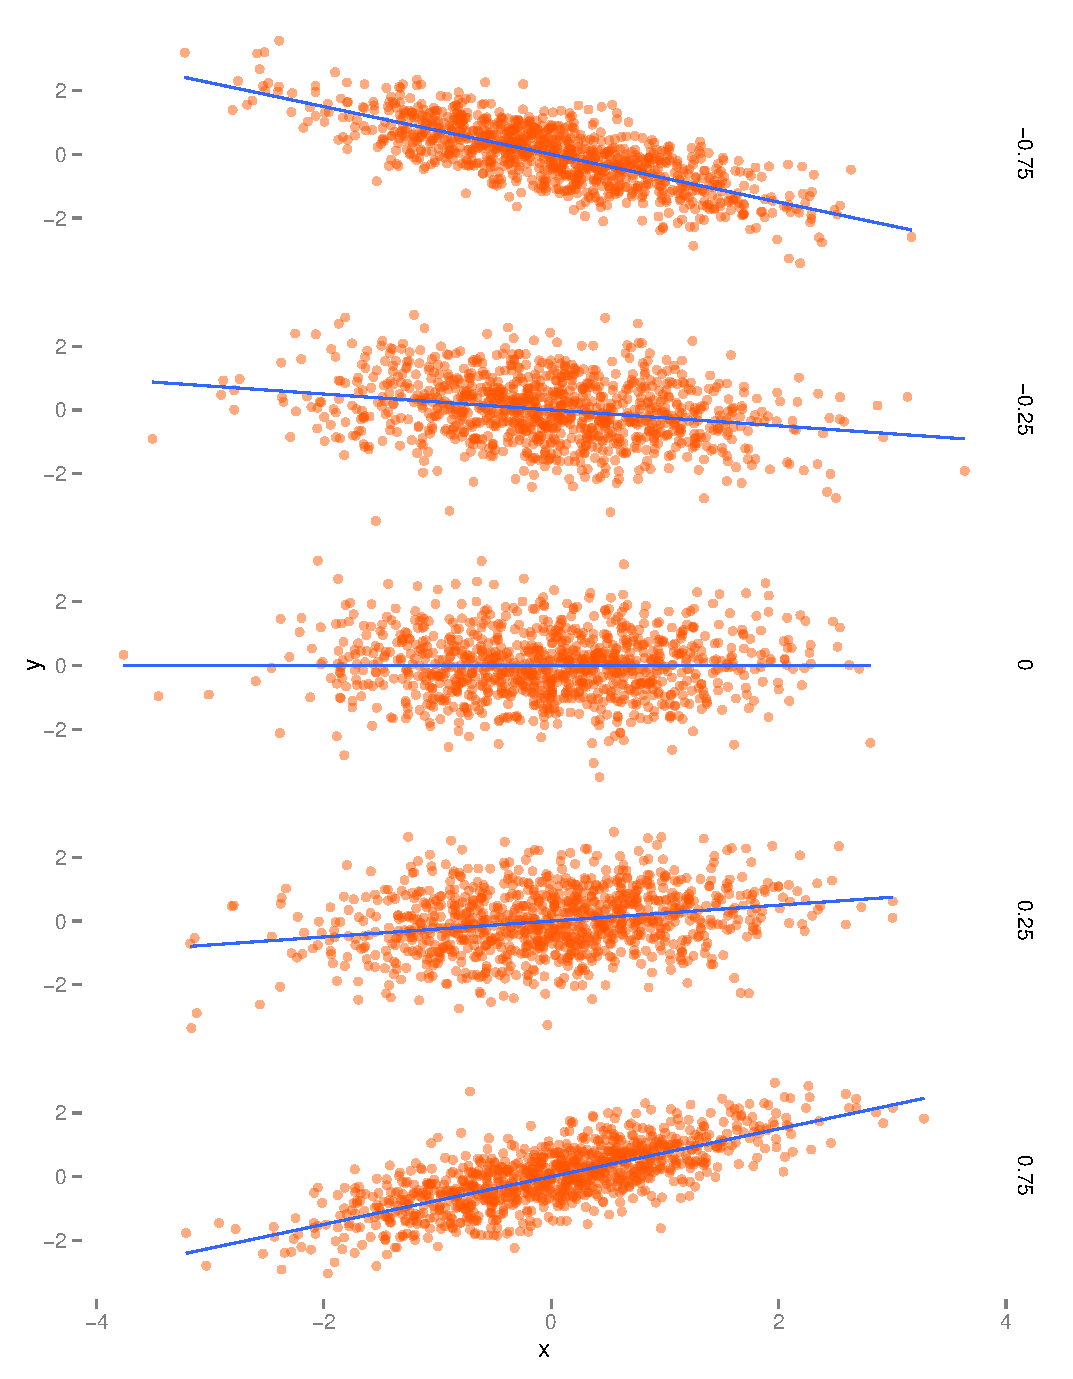
\includegraphics[scale=.25]{images/examplecors}}In the above, we have variables X and Y for which we have N paired observations. The Pearson $r$ is a standardized covariance, and ranges from -1, indicating a perfect negative linear relationship, and +1, indicating a perfect positive relationship.  A value of zero suggests no \emph{linear} association, but does not mean two variables are \emph{independent}, an extremely important point to remember.

The graph to the right shows examples of different correlations with the regression line imposed.  The following code will allow you to simulate your own.

\begin{knitrout}\footnotesize
\definecolor{shadecolor}{rgb}{0.969, 0.969, 0.969}\color{fgcolor}\begin{kframe}
\begin{alltt}
\hlfunctioncall{library}(MASS)
cormat = \hlfunctioncall{matrix}(\hlfunctioncall{c}(1, 0.25, 0.25, 1), ncol = 2)  \hlcomment{#.25 population correlation}
\hlfunctioncall{set.seed}(1234)
\hlcomment{# empirical argument will reproduce the correlation exactly if TRUE}
mydat = \hlfunctioncall{mvrnorm}(100, mu = \hlfunctioncall{c}(0, 0), Sigma = cormat, empirical = T)
\hlfunctioncall{cor}(mydat)
\end{alltt}
\begin{verbatim}
##      [,1] [,2]
## [1,] 1.00 0.25
## [2,] 0.25 1.00
\end{verbatim}
\end{kframe}
\end{knitrout}


%%%
\subsection{Spearman's Measure}
More or less just for giggles, we'll also take a look at Spearman's $\rho$.  It is essentially Pearson's $r$ on the ranked values rather than the observed values\sidenote{If you have ordinal data you might also consider using a polychoric correlation, e.g. in the \textcolor{blue}{\emph{psych}} package.}.  While it would perhaps be of use with extreme values with otherwise normally distributed data, we don't have that situation here.  However since it is a common alternative and takes no more effort to produce, it is included.


\begin{knitrout}\footnotesize
\definecolor{shadecolor}{rgb}{0.969, 0.969, 0.969}\color{fgcolor}\begin{kframe}
\begin{alltt}
\hlfunctioncall{cor}(mydat, method = \hlstring{"spearman"})  #slight difference
\end{alltt}
\begin{verbatim}
##        [,1]   [,2]
## [1,] 1.0000 0.1919
## [2,] 0.1919 1.0000
\end{verbatim}
\begin{alltt}
\hlfunctioncall{cor}(\hlfunctioncall{rank}(mydat[, 1]), \hlfunctioncall{rank}(mydat[, 2]))
\end{alltt}
\begin{verbatim}
## [1] 0.1919
\end{verbatim}
\end{kframe}
\end{knitrout}



%%%%%%%%%%%%%%%%%%%%%%%
\section{Hoeffding's D}
Hoeffding's D is another rank based approach that has been around a while\sidenote{Hoeffding (1948). A non-parametric test of independence.}. It measures the difference between the joint ranks of (X,Y) and the product of their marginal ranks. Unlike the Pearson or Spearman measures, it can pick up on nonlinear relationships, and as such would be worth examining as well.

\begin{knitrout}\footnotesize
\definecolor{shadecolor}{rgb}{0.969, 0.969, 0.969}\color{fgcolor}\begin{kframe}
\begin{alltt}
\hlfunctioncall{library}(Hmisc)
\hlfunctioncall{hoeffd}(mydat)$D
\end{alltt}
\begin{verbatim}
##         [,1]    [,2]
## [1,] 1.00000 0.01162
## [2,] 0.01162 1.00000
\end{verbatim}
\end{kframe}
\end{knitrout}


Hoeffding's D lies on the interval [-.5,1] if there are no tied ranks, with larger values indicating a stronger relationship between the variables.

%%%%%%%%%%%%%%%%%%%%%%%%%%%%%%
\section{Distance Correlation}
Distance correlation ($dCor$) is a newer measure of association \citep{szekely_measuring_2007, szekely_brownian_2009} that uses the distances between observations as part of its calculation.  

If we define a transformed distance matrix\sidenote{The standard matrix of euclidean distances with the row/column means subtracted and grand mean added.  Elements may be squared or not.}
$\mathcal{A}$ and $\mathcal{B}$ for the X and Y variables respectively, each with elements (i,j), then the distance covariance is defined as the square root of:

\medskip
$\mathcal{V}_{xy}^2 = \frac{1}{n^2}\overset{n}{\underset{i, j = 1}{\sum}} \mathcal{A}_{ij}\,\mathcal{B}_{ij}$

\medskip
and $dCor$ as the square root of

\medskip
$\mathcal{R}^2 = \frac{\mathcal{V}_{xy}^2}{\mathcal{V}_x\mathcal{V}_y}$

\medskip
Distance correlation satisfies $0 \leq \mathcal{R} \leq 1$, and $\mathcal{R} = 0$ only if X and Y are independent. In the bivariate normal case, $\mathcal{R} \leq |r|$ and equals one if $r\pm 1$ .

Note that one can obtain a $dCor$ value for X and Y of arbitrary dimension (i.e. for whole matrices, one can obtain a multivariate estimate), and one could also incorporate a rank-based version of this metric as well.

%%%%%%%%%%%%%%%%%%%%%%%%%%%%%%%%%%%%%%%%%
\section{Mutual Information and the Maximal Information Coefficient}
Touted as a 'correlation for the 21st century' (Speed, 2011), the \emph{maximal information coefficient} (MIC) is based on concepts from information theory.  We can note \emph{entropy} as a measure of uncertainty, defined for a discrete distribution with $K$ states as:

\medskip
$\mathcal{H}(X)=-\overset{k}{\underset{i=k}{\sum}} p(X=k)\log_2 p(X=k)$ \marginnote{A uniform distribution where each state was equally likely would have maximum entropy.}
\medskip

Mutual Information, a measure of how much information two variables share, then is defined as: 
\medskip

$\mathcal{I}(X;Y)=\mathcal{H}(X)+\mathcal{H}(Y)-\mathcal{H}(X,Y)$
\medskip

or in terms of conditional entropy:
\medskip

$\mathcal{I}(X;Y)=\mathcal{H}(X)-\mathcal{H}(X|Y)$
\medskip

Note that $\mathcal{I}(X;Y) = \mathcal{I}(Y;X)$. Mutual information provides the amount of information one variable reveals about another between variables of any type, ranges from 0 to $\infty$, does not depend on the functional form underlying the relationship.  Normalized variants are possible as well.

For continuous variables, the problem becomes more difficult, but if we 'bin' or \emph{discretize} the data, it then becomes possible. Conceptually we can think of placing a grid on a scatterplot of X and Y, and assign the continuous x (y) to the column (row) bin it belongs to.  At that point we can then calculate the mutual information for X and Y.
\medskip

$\mathcal{I}(X;Y)=\underset{X,Y}{\sum}p(X,Y)log_2\frac{p(X,Y)}{p(X)p(Y)}$
\medskip

\noindent With $p(X,Y)$ the proportion of data falling into bin $X,Y$, i.e. $p(X,Y)$ is the joint distribution of $X$ and $Y$.

The MIC \citep{reshef_detecting_2011} can be seen as the continuous variable counterpart to mutual information.  However, the above is seen as a na\"{i}ve estimate, and typically will overestimate $\mathcal{I}(X;Y)$.  With the MIC a search is done over various possible grids, and the MIC is the maximum $\mathcal{I}$ found over that search, with some normalization to make the values from different grids comparable.
\medskip

$MIC(X;Y)=\underset{X,Y_{total}<B}{\max}\frac{\mathcal{I}(X;Y)}{log_2(min(X,Y))}$
\medskip

In the above, $\mathcal{I}$ is the na\"{i}ve mutual information measure, which is divided by the lesser number of X or Y bins. $X,Y_{total}$ is the total number of bins, $B$ is some number, somewhat arbitrarily chosen, though \citet{reshef_detecting_2011} suggest a default of $N^{.6}$ or $N^{.55}$ based on their experiences with various data sets.

The authors make code available on \href{http://www.exploredata.net/Downloads/MINE-Application}{the web}\sidenote{See the appendix regarding an issue I found with this function.}, but just for demonstration we can use the minerva library as follows\sidenote{While the package availability is nice, the mine function in minerva works relatively very slow (even with the parallel option as in the example).}.

\begin{knitrout}\footnotesize
\definecolor{shadecolor}{rgb}{0.969, 0.969, 0.969}\color{fgcolor}\begin{kframe}
\begin{alltt}
\hlfunctioncall{library}(minerva)
\hlfunctioncall{mine}(mydat, n.cores = 3)$MIC
\end{alltt}
\begin{verbatim}
##        [,1]   [,2]
## [1,] 1.0000 0.2487
## [2,] 0.2487 1.0000
\end{verbatim}
\end{kframe}
\end{knitrout}


MIC is on the interval $[0,1]$ where zero would indicate independence and a 1 would indicate a noiseless functional relationship.  With MIC the goal is equitability- similar scores will be seen in relationships with similar noise levels regardless of the type of relationship. Because of this it may be particularly useful with high dimensional settings to find a smaller set of the strongest correlations.  Where distance correlation might be better at detecting the \emph{presence} of (possibly weak) dependencies, the MIC is more geared toward the assessment of strength and detecting patterns that we would pick up via visual inspection.



%%%%%%%%%%%%%%%%%%%%%%%%%%%%%%%
\part{Linear Relationships} %%%
%%%%%%%%%%%%%%%%%%%%%%%%%%%%%%%

Just as a grounding we will start with examination of linear relationships.  Random (standardized) normal data of size $N = 1000$ has been generated 1000 times for population correlations of -.8, -.6, -.4, 0, .4, .6, and .8 (i.e. for each correlation we create 1000 x,y data sets of $N = 1000$).  For each data set we calculate each statistic discussed above.

%%%%%%%%%%%%%%%%%
\section{Results}
Distributions of each statistic are provided in the margin\sidenote{For this and the later similar graph, rotate the document in for a better view.} (squared values for Pearson and Spearman measures). Means, standard deviations, and quantiles at the 2.5\% and 97.5\% levels are provided in the \hyperref[sec:linrel]{appendix.~\ref*{sec:linrel}} No real news to tell with the Pearson and Spearman correlations.  The other measures pick up on the relationships in a manner we'd hope, and assign the same values whether the original linear relation is positive or negative. \marginnote{\begin{flushright}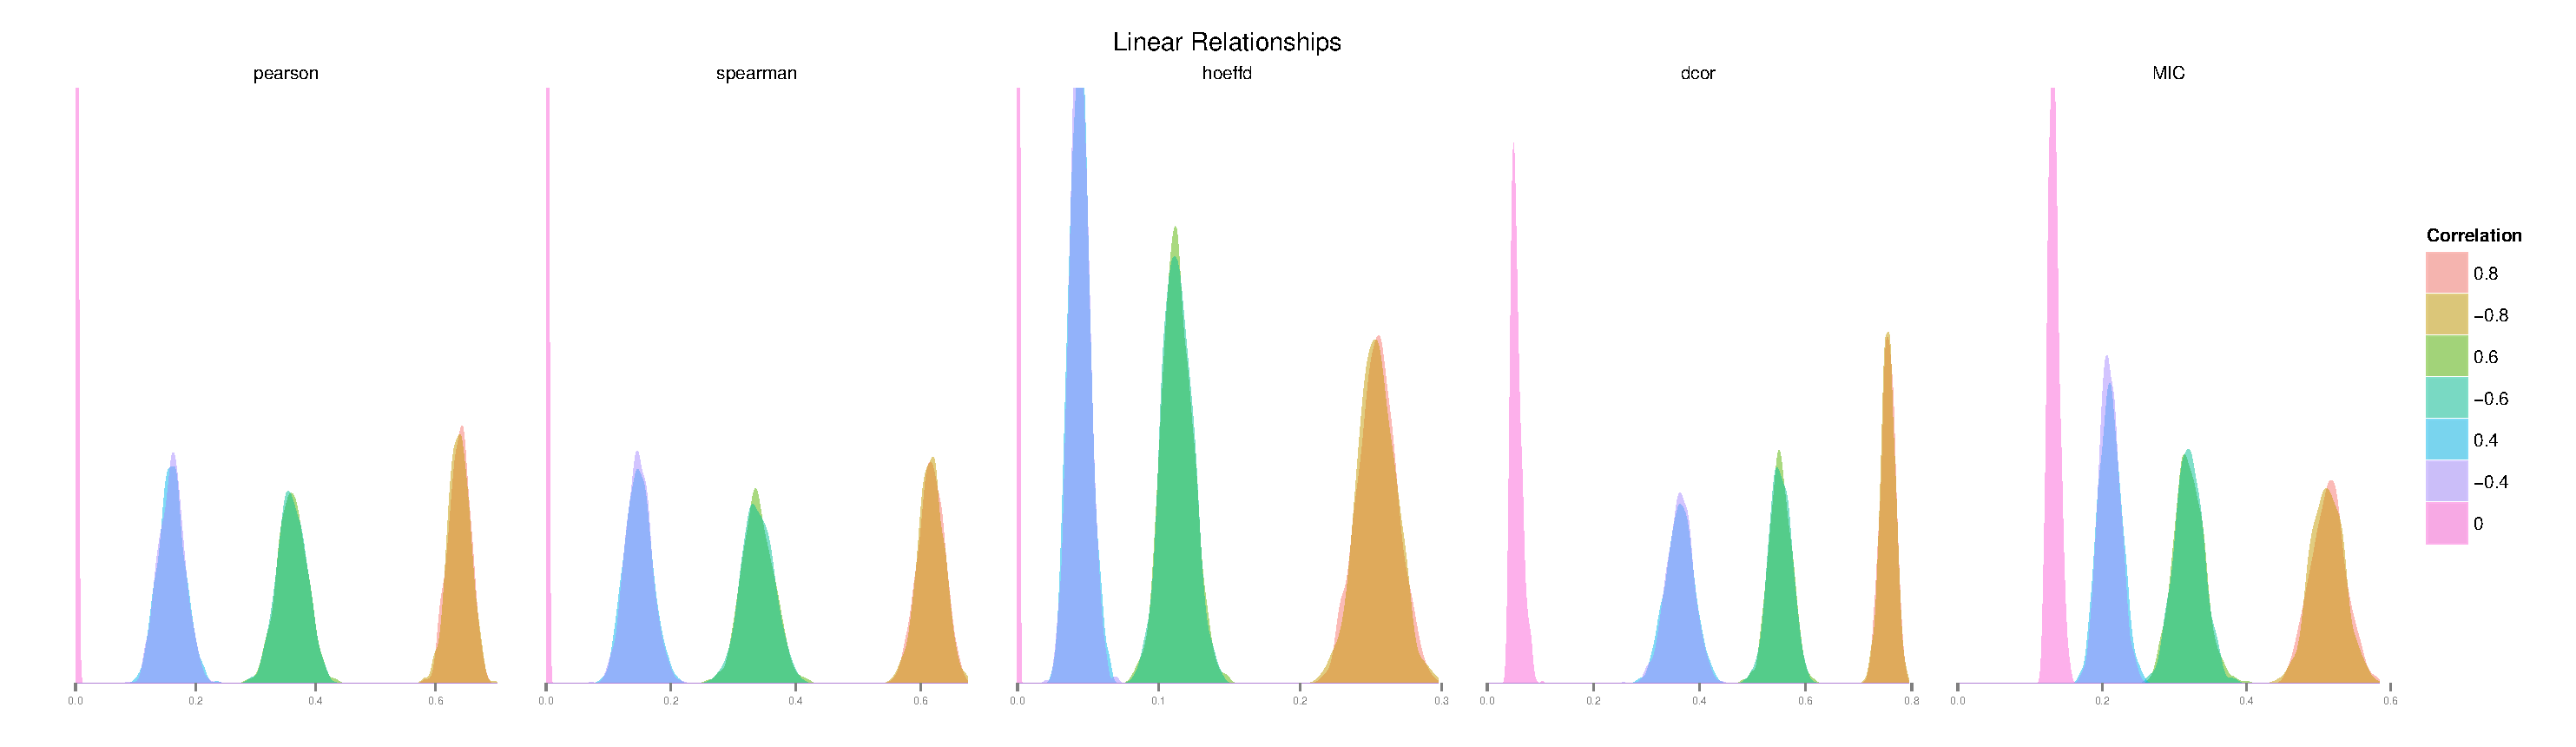
\includegraphics[scale=.25, angle=-90]{images/LinearDensities}\end{flushright}}Interestingly, the Hoeffding's D and MIC appear to get more variable as the values move away from zero, while for the $dCor$ gets less so.  At first glance  the MIC may seem to find something in nothing, in the sense it doesn't really get close to zero for the zero linear relationship.  As seen later, it finds about the same value for the same pattern split into four clusters.  This is a function of sample size, where MIC for independent data approaches  0  as $N\rightarrow\infty$.  See the supplemental material for \citet{reshef_detecting_2011}, particularly figure S1.  I also provide an example of MICs for different sample sizes and standard deviations in the \hyperref[sec:MICN0]{appendix.~\ref*{sec:MICN0}}

\marginnote{\begin{flushright}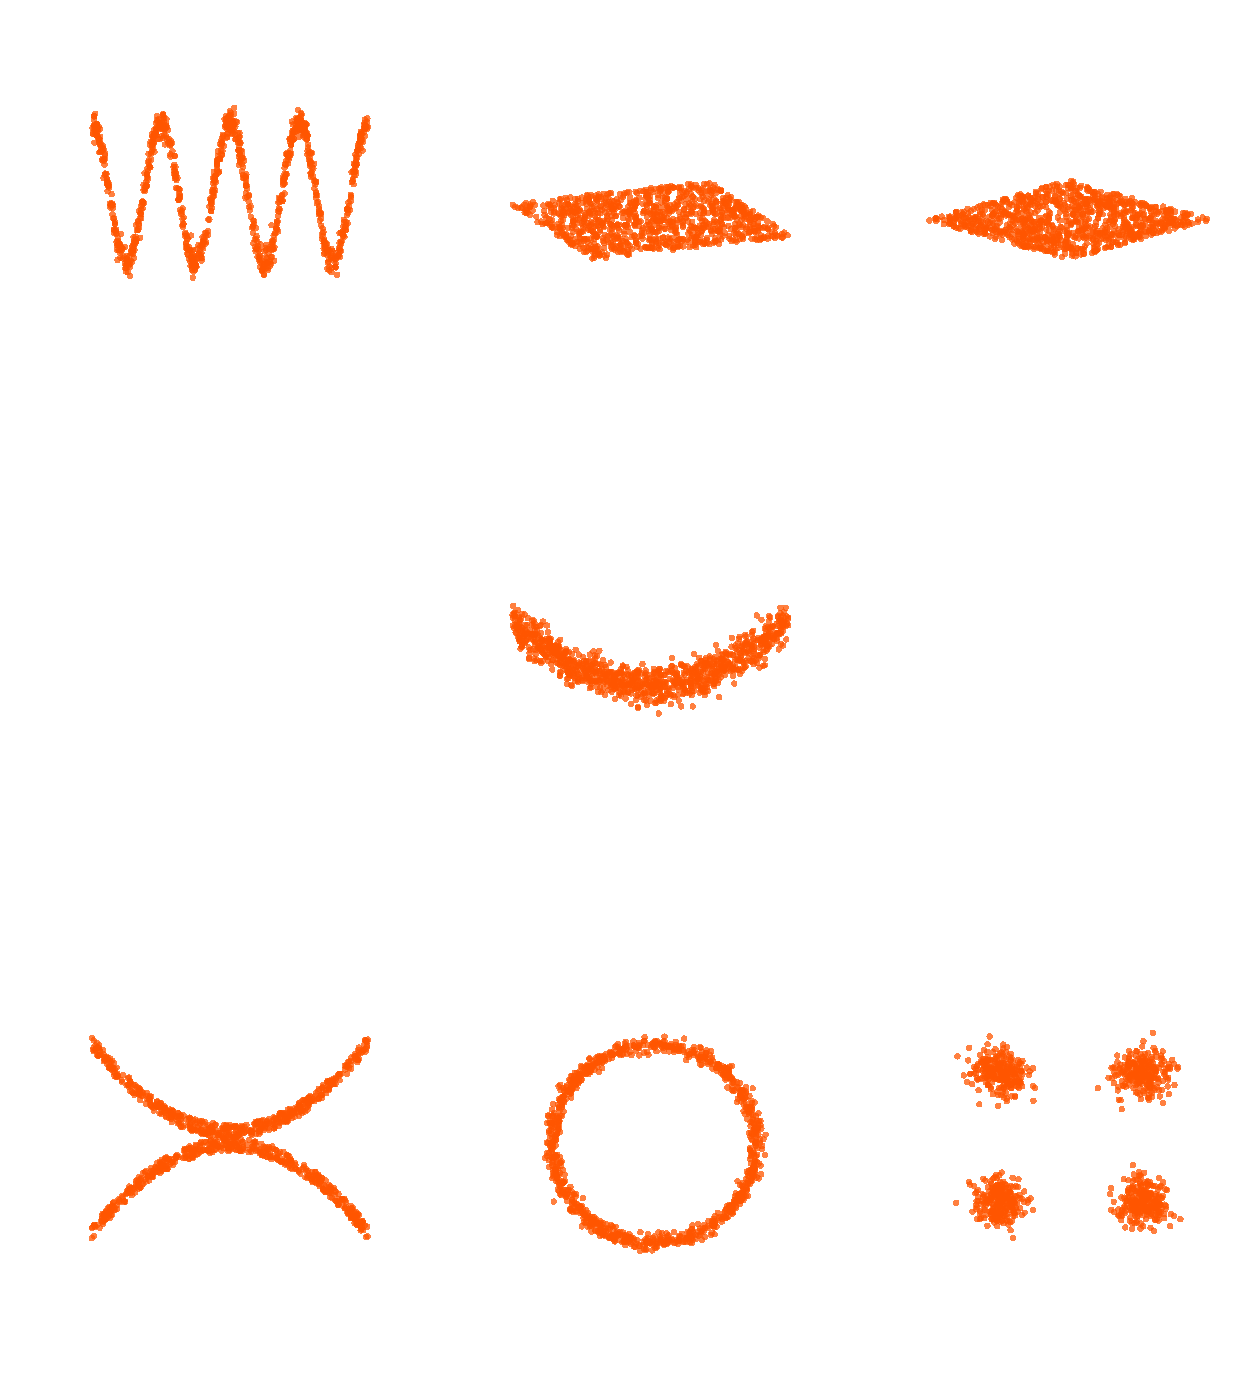
\includegraphics[scale=.2]{images/nonlinearpatternslessnoisy}\\
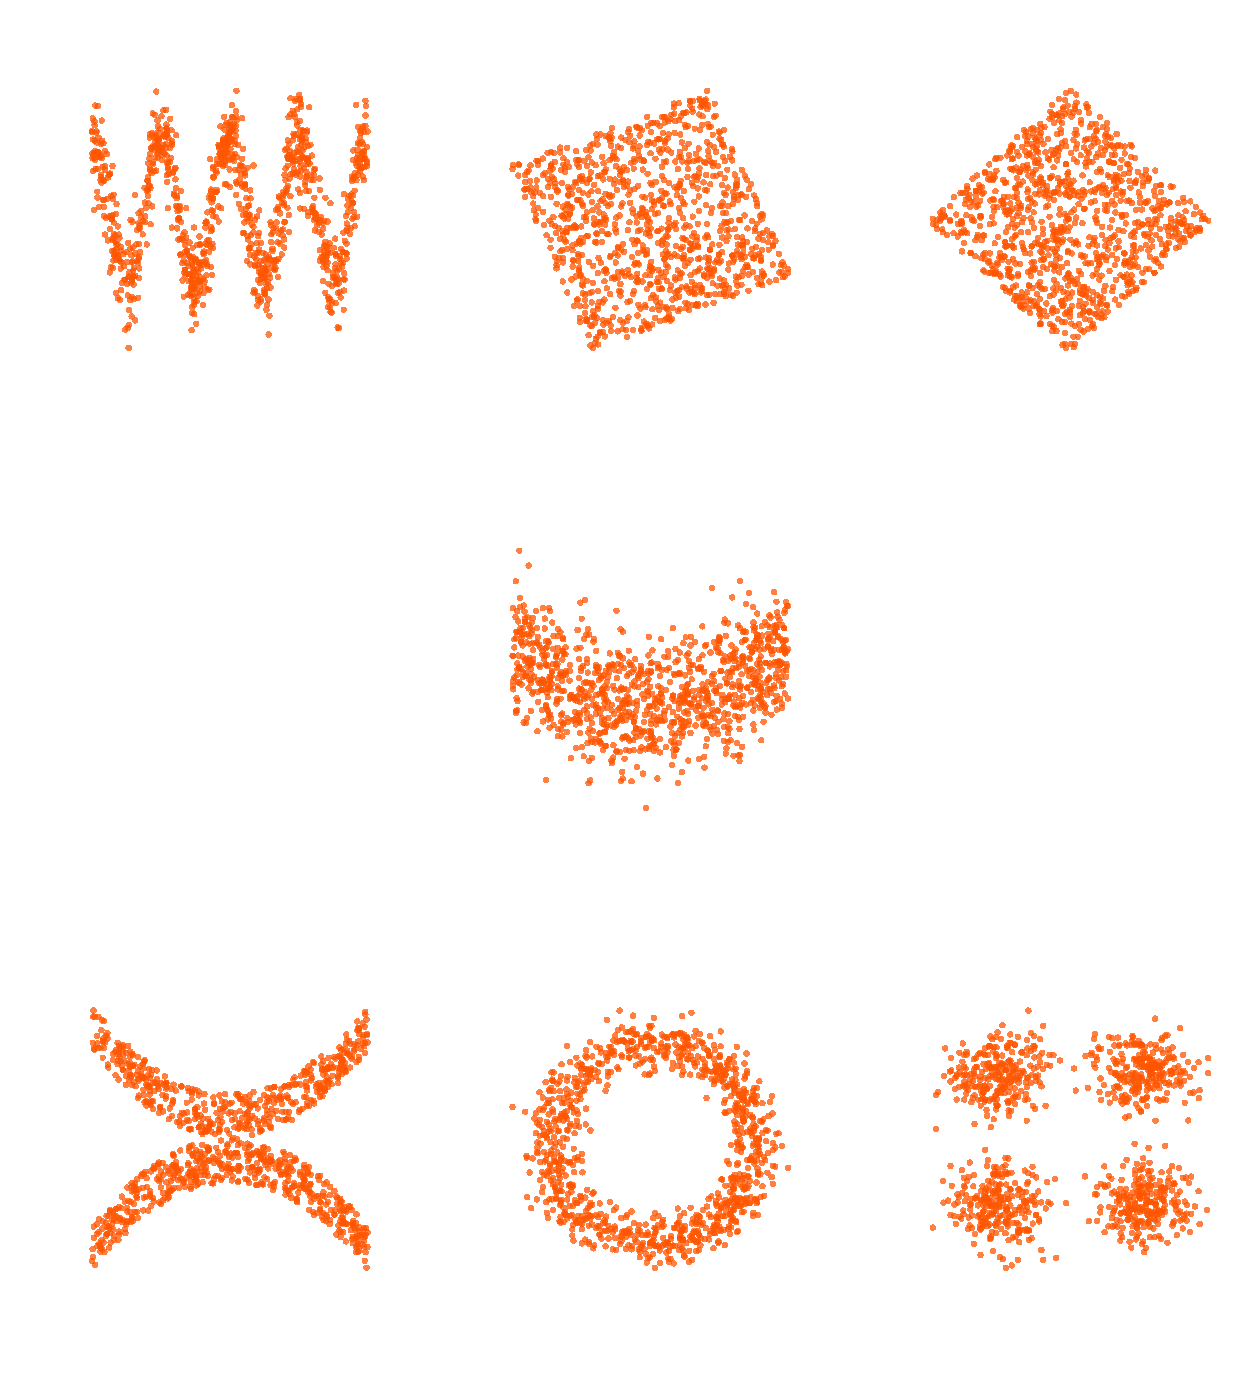
\includegraphics[scale=.2]{images/nonlinearpatternsnoisy}
\end{flushright}}
The take home message at this point is that one should feel comfortable using the other measures for standard linear relationships, as one would come to the same relative conclusions as one would with the Pearson $r$.  Note that for perfect linear relations all statistics would be 1.0. 



%%%%%%%%%%%%%%%%%%%%%%%%%%%%%%
\part{Other Relationships} %%%
%%%%%%%%%%%%%%%%%%%%%%%%%%%%%%

More interesting is a comparison of these alternatives when the relationship is not linear. To this end, seven other patterns are investigated to see how these statistics compare.  In the margin are examples of the patterns at two different noise levels.  The patterns will be referred to as wave, trapezoid, diamond, quadratic, X, circle and cluster.

%%%%%%%%%%%%%%%%%
\section{Results}

Distributional results for the distance correlation and MIC can again be seen in the margin, related statistics and distributions for the those and the other statistics can be found in the \hyperref[sec:nonlinrel]{appendix.~\ref*{sec:nonlinrel}}  Neither Pearson's $r$ nor Spearman's $\rho$ find a relationship among any of the patterns regardless of noise level, and will no longer be a point of focus.  


%%%
\subsection{Less noisy}
Hoeffding's D shows very little variability within its estimates for any particular pattern, and does not vary much between patterns (means range 0 to .1).  In this less noisy situation Hoeffding's D does pick up on the quadratic pattern relative to the others, followed by the X and circle patterns, but in general these are fairly small values for any pattern. 


The $dCor$ and MIC show notable values for most of these patterns.  The $dCor$ finds the strongest relationship for the quadratic function, followed by the X, circle, the trapezoidal and wave patterns in a group, with the cluster pattern near zero. \marginnote{\raggedleft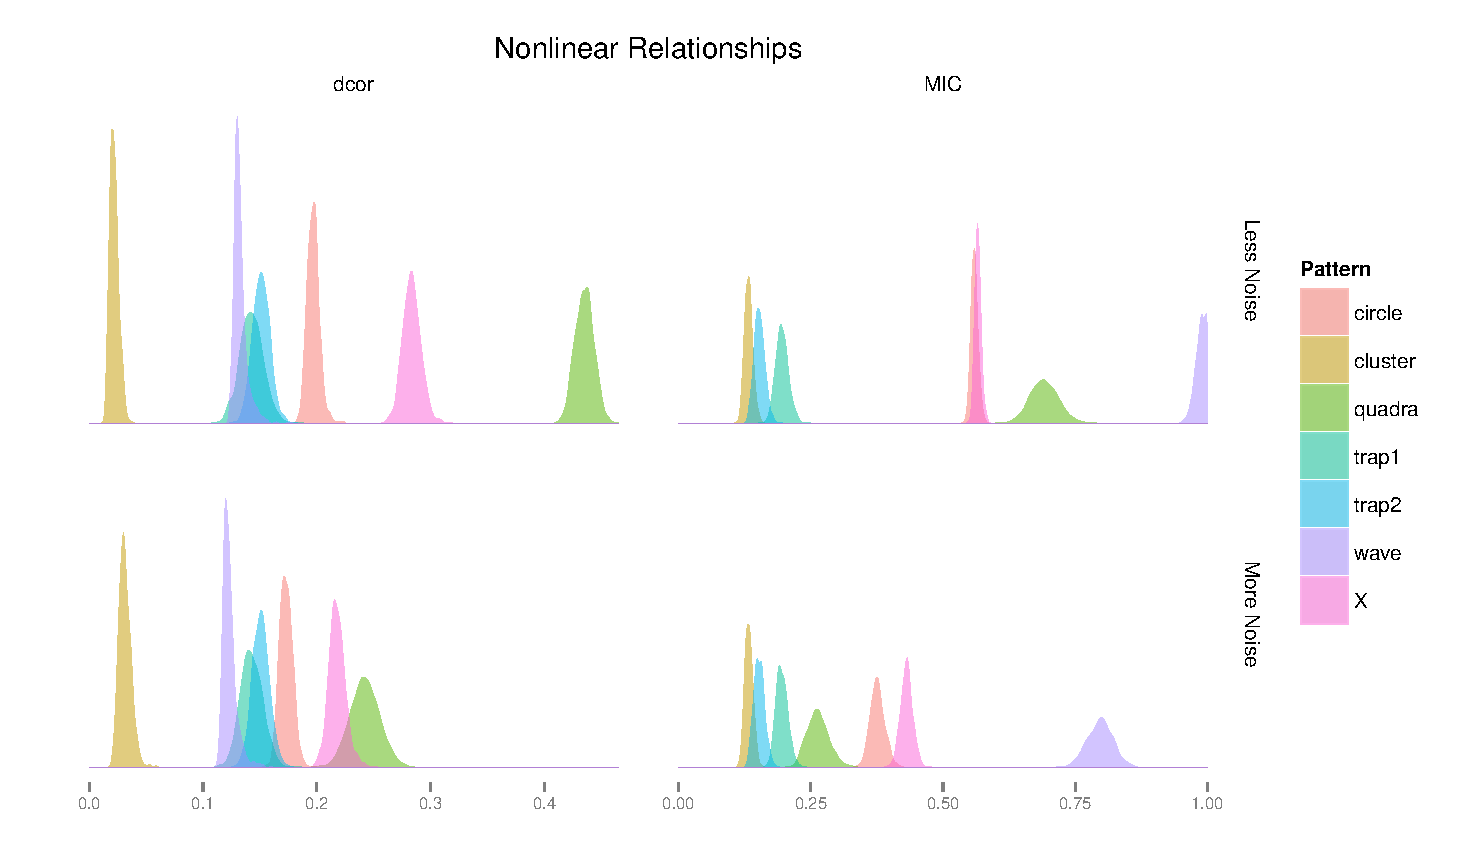
\includegraphics[scale=.45, angle=-90]{images/NonlinearDensitiesdcorMIC}}The MIC finds a very strong relationship for the wave pattern, followed by the quadratic, about the same for the circle and X pattern, and the rest filling out toward its lower values.  Just as before, the MIC won't quite reach 0 for $N = 1000$, so those last three are probably reflective of little dependence according to MIC.


%%%
\subsection{Noisier}
With more noise, Hoeffding's D does not pick up on the patterns well; the means now range from 0 to .02. The $dCor$ maintains its previous ordering, although in general the values are smaller, or essentially the same in the case of the trapezoidal and cluster patterns for which strong dependency was not uncovered previously. The MIC still finds a strong dependency in the wave pattern, as well as the X and circle, but the drop off for the quadratic relationship is notable, and is now deemed less of a dependency than the circle and X patterns.  The remaining are essentially the same as the less noisy situation.  This suggests that for some relationships the MIC will produce the same value regardless of the amount of noise, and the noise level may affect the ordering of the strength one would see of different relationships.



%%%%%%%%%%%%%%%%%%%%%
\part{Summary} %%%
%%%%%%%%%%%%%%%%%%%%%
Pearson's $r$ and similar measures are not designed to pick up nonlinear relationships or dependency in a general sense.  Other approaches such as Hoeffding's D might do a little better in some limited scenarios, and a statistical test\sidenote{The \textcolor{red}{hoeffd} function does return a p-value if interested.} for it might suggest dependence given a particular nonlinear situation.  However it appears one would not get a good sense of the strength of that dependence, nor would various patterns of dependency be picked up.  It also does not have the sort of properties the MIC is attempting to hold.

Both distance correlation and MIC seem up to the challenge to find dependencies beyond the linear realm. However neither is perfect, and \citet{kinney_equitability_2013} note several issues with MIC in particular.  They show that MIC is actually not equitable\sidenote{The $R^2$ measure of equitabilitity Reshef et al. were using doesn't appear to be a useful way to measure it either.}, the key property Reshef and co. were claiming, nor is it 'self-equitable' either (neither is $dCor$).  Kinney and Atwal also show, and we have seen here, that variable noise may not affect the MIC value for certain relationships, and they further note that one could have a MIC of 1.0 for differing noise levels.

As for distance correlation, Simon and Tibshirani (2011, see \hyperref[sec:addinfo]{additional information~\ref*{sec:addinfo}} for a link to their comment) show that $dCor$ exhibits more statistical power than the MIC.  We have also seen it will tend to zero even with smaller sample sizes, and that it preserved the ordering of dependencies found across noise levels.  Furthermore, $dCor$ is straightforward to calculate and not an approximation.  

In the end we may still need to be on the lookout for a measure that is both highly interpretable and possesses all the desirable qualities we want, but we certainly have do have measures that are viable already. \citet{kinney_equitability_2013} suggest that the issues surrounding mutual information $\mathcal{I}$ that concern Reshef et al. were more a sample size issue, and that those difficulties vanish with very large amounts of data.  For smaller sample sizes and/or to save computational costs, Kinney and Atwal suggest $dCor$ would be a viable approach.

\vspace{1cm}
I think the most important conclusion to draw is to try something new.  Pearson's simply is not viable for understanding a great many dependencies that one will regularly come across in one's data adventures. Both $dCor$ and mutual information seem much better alternatives for picking up on a wide variety of relationships that variables might exhibit, and can be as useful as our old tools.  Feel free to experiment!



\newpage

%%%%%%%%%%%%%%%%%%%
\part{Appendix} %%%
%%%%%%%%%%%%%%%%%%%

\section{Mine Results}
Note on the rMine code available at \href{http://www.exploredata.net/Downloads/MINE-Application}{http://www.exploredata.net/
Downloads/MINE-Application}. I have come across a couple of issues.  One is that it will simply not work (as the Tibshirani comment refers to it, a 'glitch'), producing a missing value.  But in addition to that, I found that it also appears to produce odd values every once in a while.  Consider the following graphs in which various notably high linear relationships are examined, with the rMine function and the \textcolor{red}{mine} function from the \textcolor{blue}{\emph{minerva}} respectively.  The rMine function bounces around quite a bit, even tending toward very low values on regular occasion, although the peak of the distribution is about right. In contrast the minerva function shows more symmetric and stable distributions, even with a little bit of bump in the tails.  The rMine code was beta and dated Jan. 2012, so it may have changed by the time you play with it. 



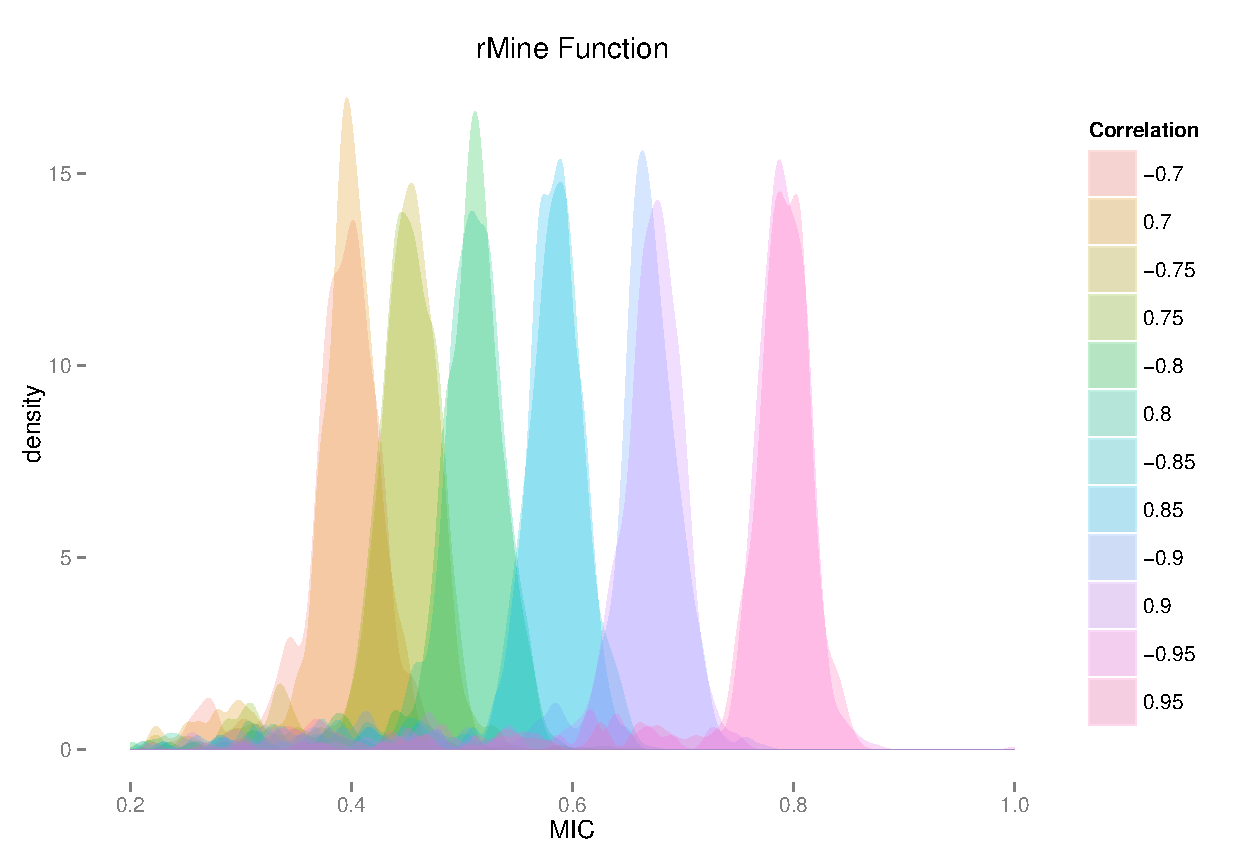
\includegraphics[scale=.30]{images/MICDensitiesHiCorr_mymine}

\vspace{.25cm}
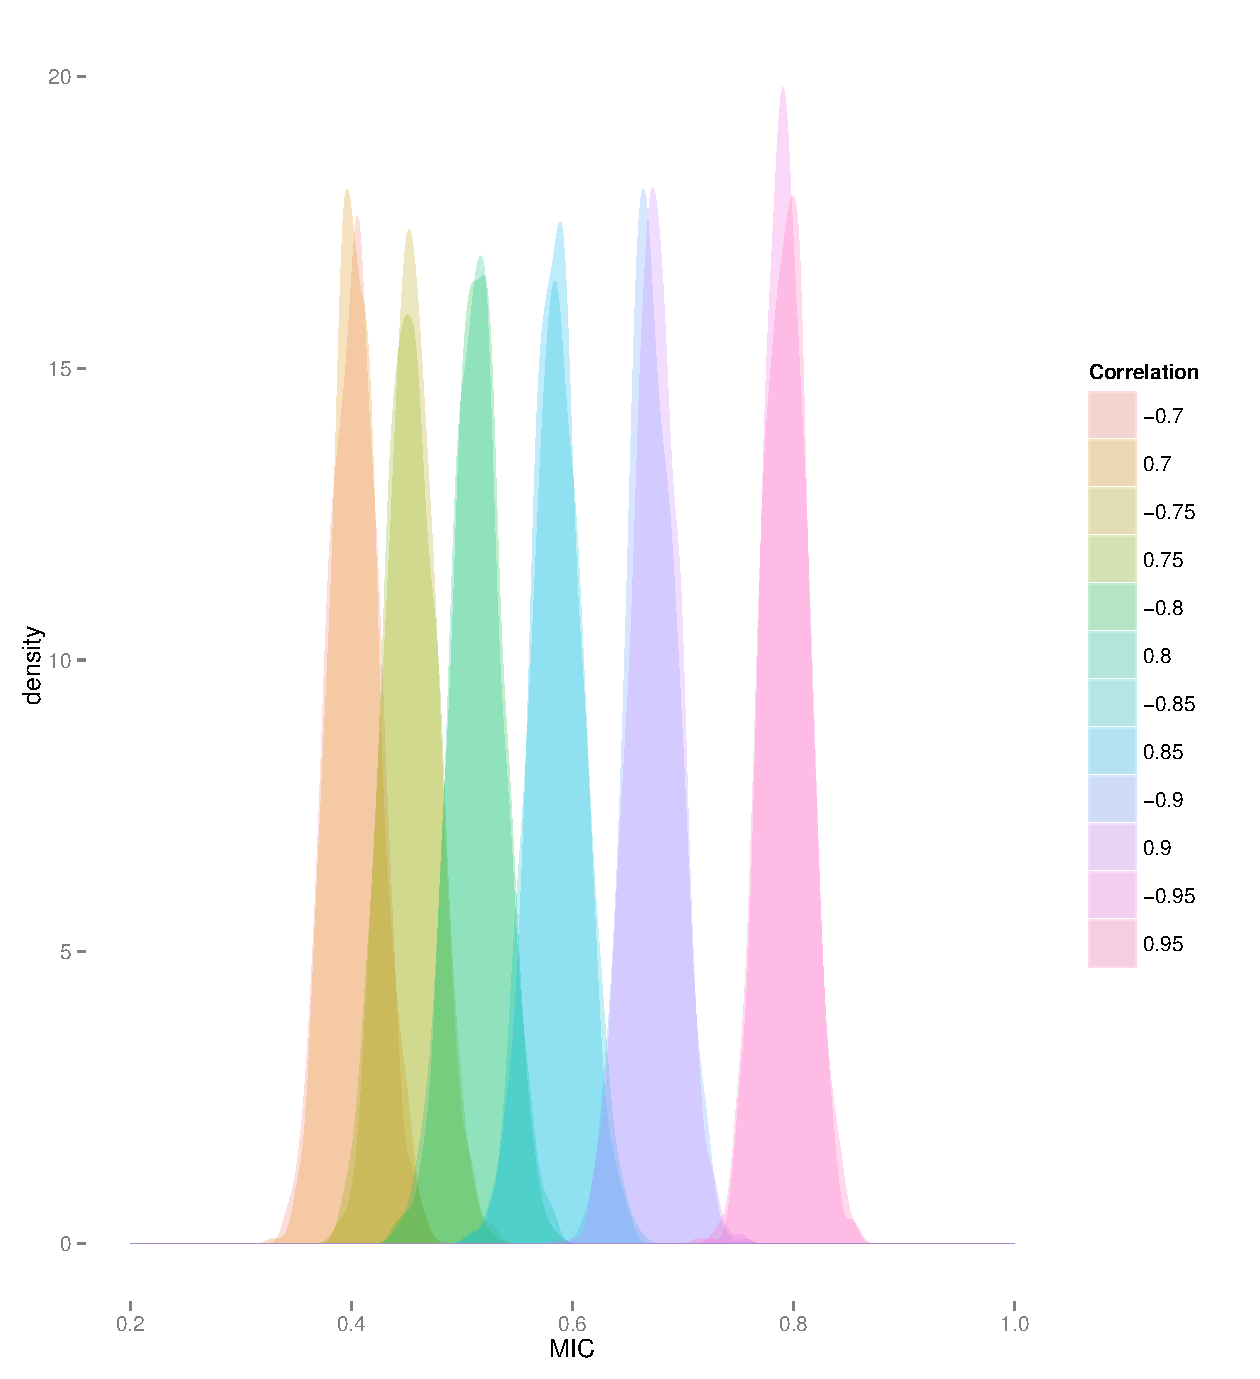
\includegraphics[scale=.30]{images/MICDensitiesHiCorr}


%%%%%%%%%%%%%%%%%%%%%%%%%%%%%%%%%%%%%%%%%%
\section{Statistics: Linear Relationships}\label{sec:linrel}
 
\footnotesize{
\indent Means.\\
\begin{tabular}{rrrrrr}
pop. & pearson & spearman & hoeffd  & dcor & MIC \\
\hline
.8 & 0.799 & 0.785 & 0.255 & 0.755 & 0.513 \\
.6 & 0.600 & 0.582 & 0.113 & 0.552 & 0.321 \\
.4 & 0.399 & 0.383 & 0.044 & 0.363 & 0.211 \\
0 & -0.001 & -0.001 & 0.000 & 0.055 & 0.133 \\
-.4 & -0.399 & -0.384 & 0.044 & 0.363 & 0.210 \\
-.6 & -0.600 & -0.582 & 0.113 & 0.552 & 0.320 \\
-.8 & -0.799 & -0.785 & 0.254 & 0.755 & 0.512 \\
\hline
\end{tabular}

\vspace{.25cm}
\noindent Standard deviations.\\
\begin{tabular}{rrrrrr}
pearson & spearman & hoeffd & dcor & MIC  \\
\hline
0.011 & 0.013 & 0.014 & 0.013 & 0.024  \\
0.020 & 0.022 & 0.011 & 0.021 & 0.021  \\
0.027 & 0.028 & 0.007 & 0.026 & 0.016  \\
0.031 & 0.031 & 0.000 & 0.010 & 0.007  \\
0.027 & 0.027 & 0.007 & 0.025 & 0.014  \\
0.020 & 0.022 & 0.011 & 0.021 & 0.020  \\
0.012 & 0.013 & 0.014 & 0.013 & 0.023  \\
\hline
\end{tabular}

\vspace{.25cm}
\noindent Quantiles at the 2.5\% and 97.5\% levels.\\
\begin{tabular}{rrrrr}

pearson & spearman & hoeffd & dcor & MIC  \\ 
\hline \relax %b/c latex is idiotic with brackets
[0.777 0.820] & [0.758 0.810] & [0.228 0.282] & [0.729 0.780] & [0.467 0.560] \\ \relax
[0.560 0.640] & [0.540 0.624] & [0.093 0.135] & [0.513 0.593] & [0.281 0.366] \\ \relax
[0.345 0.452] & [0.328 0.439] & [0.031 0.059] & [0.311 0.416] & [0.182 0.242] \\ \relax
[-0.062  0.060] & [-0.062 0.058] & [0.000 0.001] & [0.040 0.080] & [0.120 0.149] \\ \relax
[-0.449 -0.344] & [-0.436 -0.327] & [0.030 0.058] & [0.309 0.412] & [0.183 0.240] \\ \relax
[-0.638 -0.561] & [-0.624 -0.538] & [0.093 0.135] & [0.509 0.592] & [0.282 0.360] \\ \relax
[-0.821 -0.775] & [-0.810 -0.757] & [0.226 0.281] & [0.726 0.780] & [0.466 0.558] \\
\hline
\end{tabular}
}


\vspace{2.5cm}
%%%%%%%%%%%%%%%%%%%%%%%%%%%%%%%%%%%%%%%%%%%%%%%%%%%%
\section{MIC tends toward zero for independent data}\label{sec:MICN0}
MIC for x and y random draws of size N and $N(0, sd)$.\\

\footnotesize{
\begin{tabular}{lrrrr}
N  & 10 & 1 & 0.1 & 0.01 \\
\hline
100 & 0.251 & 0.263 & 0.228 & 0.255 \\
500 & 0.166 & 0.146 & 0.150 & 0.160 \\
1000 & 0.144 & 0.137 & 0.133 & 0.144 \\
2500 & 0.097 & 0.095 & 0.101 & 0.101 \\
5000 & 0.084 & 0.078 & 0.082 & 0.079 \\
10000 & 0.064 & 0.065 & 0.062 & 0.063 \\
20000 & 0.050 & 0.046 & 0.046 & 0.045 \\
\hline
\end{tabular}
}


%%%%%%%%%%%%%%%%%%%%%%%%%%%%%%%%%%%%%%%%%%%%%
\section{Statistics: Nonlinear Relationships}\label{sec:nonlinrel}
\subsection{Pearson and Spearman Distributions}
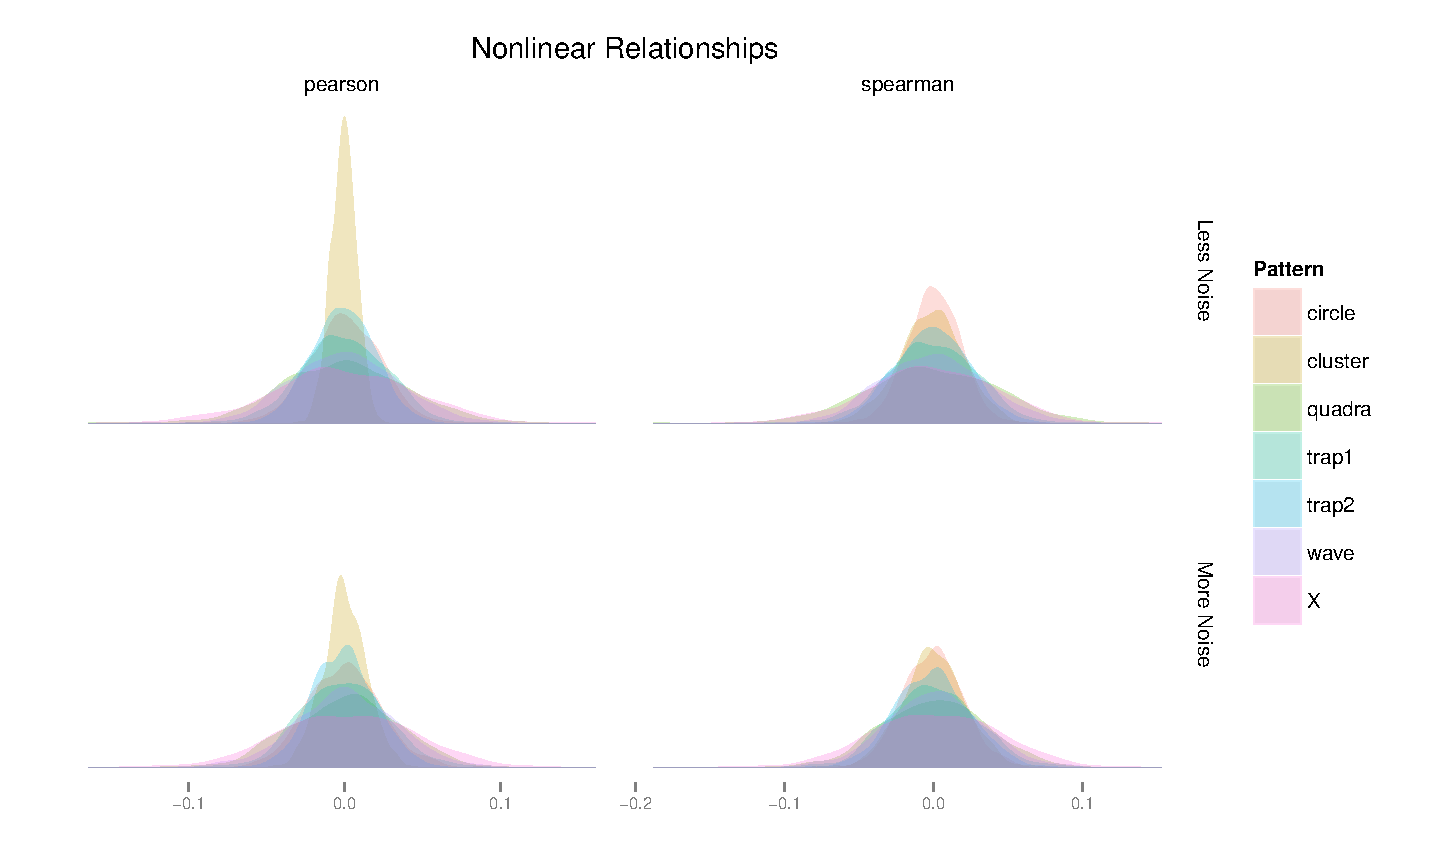
\includegraphics[scale=.5]{images/NonlinearDensitiespearsonspearman}

\subsection{Hoeffding's D Distributions}
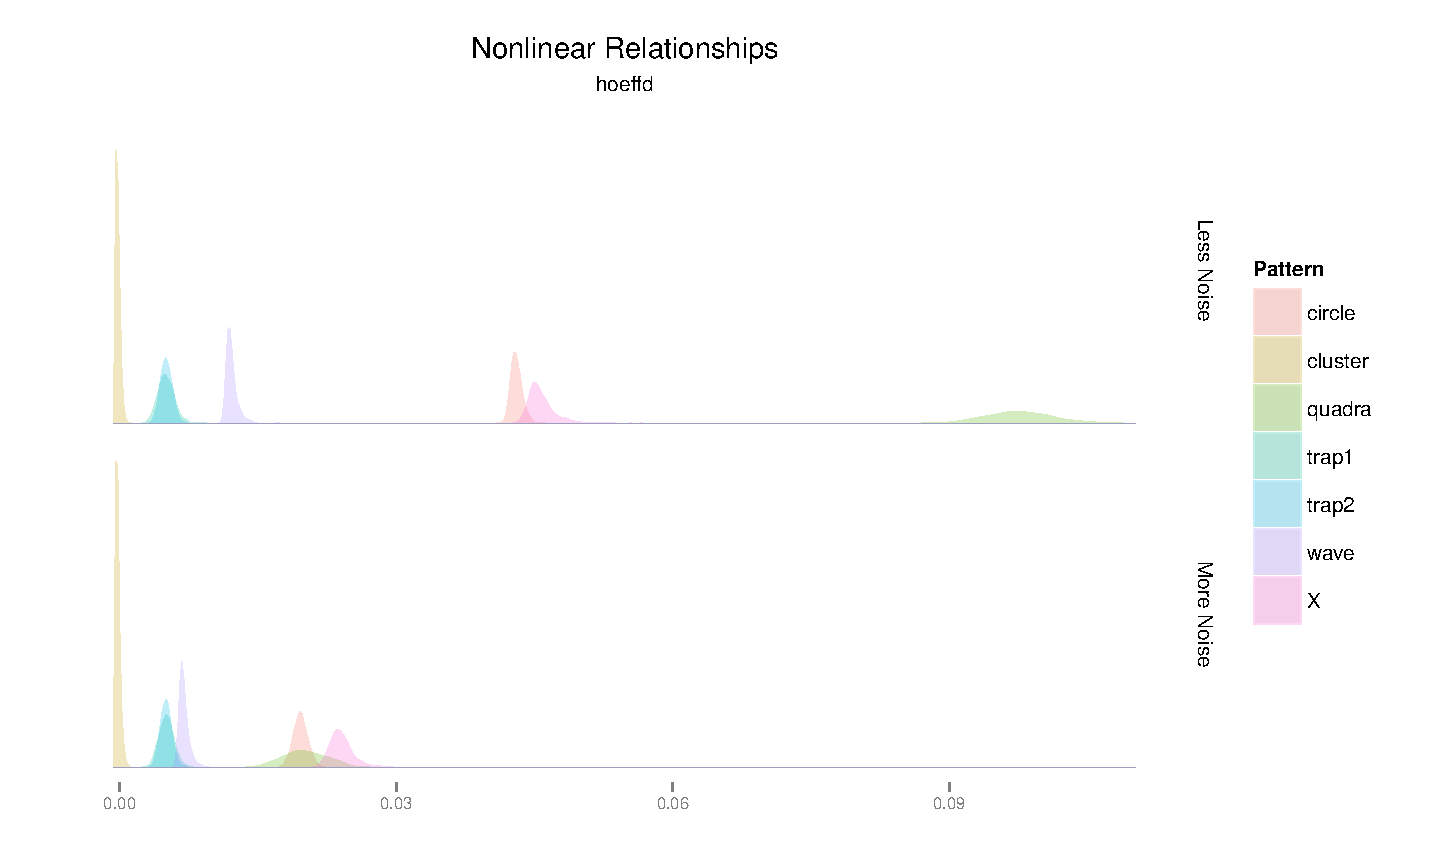
\includegraphics[scale=.5]{images/NonlinearDensitieshoeffd}


\newpage
%%%
\subsection{Less Noisy Patterns}

\footnotesize{
Means.\\
\begin{tabular}{lrrrrr}

pattern & pearson & spearman & hoeffd & dcor & MIC \\
\hline
\emph{wave} & 0.000 & 0.000 & 0.012 & 0.132 & 0.988 \\
\emph{trapezoid} & -0.001 & -0.001 & 0.005 & 0.143 & 0.196 \\
\emph{diamond} & -0.001 & -0.001 & 0.005 & 0.151 & 0.153 \\
\emph{quadra} & 0.000 & -0.001 & 0.098 & 0.435 & 0.692 \\
\emph{X} & -0.001 & -0.001 & 0.046 & 0.283 & 0.566 \\
\emph{circle} & 0.000 & 0.000 & 0.043 & 0.197 & 0.560 \\
\emph{cluster} & -0.001 & -0.002 & 0.000 & 0.022 & 0.133 \\
\hline
\end{tabular}

\vspace{.25cm}
\noindent Standard deviations.\\
\begin{tabular}{lrrrrr}
pattern & pearson & spearman & hoeffd & dcor & MIC \\
\hline
\emph{wave} & 0.033 & 0.034 & 0.001 & 0.006 & 0.010 \\
\emph{trapezoid} & 0.027 & 0.029 & 0.001 & 0.010 & 0.012 \\
\emph{diamond} & 0.020 & 0.024 & 0.001 & 0.007 & 0.010 \\
\emph{quadra} & 0.039 & 0.042 & 0.004 & 0.008 & 0.026 \\
\emph{X} & 0.044 & 0.042 & 0.002 & 0.008 & 0.006 \\
\emph{circle} & 0.022 & 0.018 & 0.001 & 0.005 & 0.007 \\
\emph{cluster} & 0.008 & 0.021 & 0.000 & 0.004 & 0.008 \\
\hline
\end{tabular}


\vspace{.25cm}
\noindent Quantiles at the 2.5\% and 97.5\% levels.\\

\begin{tabular}{lrrrrr}
pattern & pearson & spearman & hoeffd & dcor & MIC  \\ 
\hline  \relax 
\emph{wave}   & [-0.062 0.064] & [-0.062 0.068] & [0.011 0.014] & [0.125 0.148] & [0.965 1.000]  \\ \relax 
\emph{trapezoid}  & [-0.053 0.048] & [-0.057 0.053] & [0.003 0.007] & [0.123 0.163] & [0.174 0.221]  \\ \relax
\emph{diamond}  & [-0.040 0.037] & [-0.048 0.047] & [0.004 0.006] & [0.137 0.166] & [0.135 0.174]  \\ \relax
\emph{quadra} & [-0.074 0.076] & [-0.083 0.083] & [0.091 0.105] & [0.420 0.451] & [0.642 0.746]  \\ \relax
\emph{X}      & [-0.093 0.084] & [-0.085 0.077] & [0.044 0.050] & [0.269 0.299] & [0.556 0.578]  \\ \relax
\emph{circle} & [-0.043 0.042] & [-0.034 0.034] & [0.042 0.044] & [0.188 0.208] & [0.548 0.573]  \\ \relax
\emph{cluster} & [-0.017 0.014] & [-0.045 0.039] & [-0.001 0.000] & [0.016 0.030] & [0.119 0.149]\\
\hline
\end{tabular}
}



\pagebreak
%%%
\subsection{Noisier Patterns}
{\footnotesize
Means.\\
\begin{tabular}{lrrrrr}
pattern & pearson & spearman & hoeffd & dcor & MIC \\
\hline
\emph{wave} &  0.001 & 0.001 & 0.007 & 0.123 & 0.797 \\
\emph{trapezoid} & -0.001 & 0.000 & 0.005 & 0.143 & 0.196 \\
\emph{diamond} &  0.000 & -0.001 & 0.005 & 0.151 & 0.153 \\
\emph{quadra} & 0.000 & 0.000 & 0.020 & 0.242 & 0.264 \\
\emph{X}   & 0.001 & 0.001 & 0.024 & 0.218 & 0.431 \\
\emph{circle} & 0.000 & 0.000 & 0.020 & 0.173 & 0.376 \\
\emph{cluster} & 0.000 & 0.000 & 0.000 & 0.032 & 0.133 \\
\hline
\end{tabular}

\vspace{.25cm}
\noindent Standard deviations.\\
\begin{tabular}{lrrrrr}
pattern & pearson & spearman & hoeffd & dcor & MIC \\
\hline
\emph{wave} & 0.032 & 0.032 & 0.001 & 0.006 & 0.024 \\
\emph{trapezoid} & 0.027 & 0.029 & 0.001 & 0.010 & 0.011 \\
\emph{diamond} & 0.020 & 0.024 & 0.001 & 0.007 & 0.010 \\
\emph{quadra} & 0.033 & 0.034 & 0.002 & 0.013 & 0.021 \\
\emph{X} & 0.043 & 0.042 & 0.001 & 0.007 & 0.011 \\
\emph{circle} & 0.023 & 0.020 & 0.001 & 0.006 & 0.013 \\
\emph{cluster} & 0.014 & 0.021 & 0.000 & 0.005 & 0.008 \\
\hline
\end{tabular}


\vspace{.25cm}
\noindent Quantiles at the 2.5\% and 97.5\% levels.\\
\begin{tabular}{lrrrrr}
pattern & pearson & spearman & hoeffd & dcor & MIC  \\ 
\hline \relax %b/c latex is idiotic with brackets
\emph{wave}      &    [-0.066         0.062] & [-0.063          0.063] & [0.006        0.008] & [0.116      0.139] & [0.750     0.843]\\ \relax
\emph{trapezoid}     &    [-0.049         0.053] & [-0.052          0.054] & [0.004        0.007] & [0.124      0.162] & [0.176     0.219]\\ \relax
\emph{diamond}     &    [-0.038         0.039] & [-0.048          0.049] & [0.004        0.006] & [0.137      0.166] & [0.135     0.173]\\ \relax
\emph{quadra}    &    [-0.061         0.063] & [-0.065          0.066] & [0.016        0.025] & [0.218      0.268] & [0.229     0.307]\\ \relax
\emph{X}         &    [-0.080         0.084] & [-0.078          0.080] & [0.022        0.028] & [0.204      0.235] & [0.409     0.454]\\ \relax
\emph{circle}    &    [-0.043         0.048] & [-0.038          0.042] & [0.018        0.021] & [0.163      0.185] & [0.352     0.403]\\ \relax
\emph{cluster}   &    [-0.028         0.027] & [-0.040          0.041] & [-0.001        0.000] & [0.023      0.043] & [0.120     0.148]\\
\hline
\end{tabular}
}


\pagebreak


\bibliography{corrmeasbib} %corrmeasbibwithtibs.tex
%\normalsize{}

\nocite{szekely_measuring_2007}
\nocite{szekely_brownian_2009}
\nocite{reshef_detecting_2011}
\nocite{fujita_comparing_2009}
\nocite{reshef_equitability_2013}
\nocite{kinney_equitability_2013}
\nocite{simontibs_2011}
\nocite{heller_consistent_2012}

\normalsize

%%%%%%%%%%%%%%%%%%%%%%%%%%%%%%%%
\section{Additional Information}\label{sec:addinfo}
Some R packages to calculate mutual information (package names linked):

\noindent\href{http://www.bioconductor.org/packages/2.12/bioc/html/minet.html}{\textcolor{blue}{\emph{minet}}}: implements various algorithms for inferring mutual information networks from data\sidenote{Via the Bioconductor repository.}\\
\noindent\href{http://cran.r-project.org/web/packages/infotheo}{\textcolor{blue}{\emph{infotheo}}}: for continuous variables requires discretization via \textcolor{red}{discretize} function \\
\noindent\href{http://r-forge.r-project.org/projects/mpmi/}{\textcolor{blue}{\emph{mpmi}}}: Fast calculation mutual information for comparisons between all types of variables including continuous vs continuous, continuous vs discrete and discrete vs discrete.

\medskip
\noindent R package to calculate distance correlation (package names linked):
\noindent\href{http://cran.r-project.org/web/packages/energy/}{\textcolor{blue}{\emph{energy}}}: E-statistics (energy) tests and statistics for comparing distributions. From Sz\'{e}kely and Rizzo, authors of the papers cited.

\medskip
\noindent R package for the \href{http://www.math.tau.ac.il/~ruheller/Software.html}{HHG} measure of association/test; provided by the cited author.  I may come back to this in a future version of this paper.

\medskip
\noindent Commentary for \citet{reshef_detecting_2011} at article \href{http://comments.sciencemag.org/content/10.1126/science.1205438}{website}.

\medskip
\noindent Some discussion at Andrew Gelman's blog (\href{http://andrewgelman.com/2011/12/16/mr-pearson-meet-mr-mandelbrot-detecting-novel-associations-in-large-data-sets/}{1}) (\href{http://andrewgelman.com/2012/03/26/further-thoughts-on-nonparametric-correlation-measures/}{2}) 
\medskip

\noindent Simon and Tibshirani's \href{http://www-stat.stanford.edu/~tibs/reshef/comment.pdf}{comment}.
\medskip


\noindent The code I used for this paper was a modification of that available both at \href{http://www-stat.stanford.edu/~tibs/reshef/script.R}{Tibshirani's website}, and code available for the patterns seen at the \href{http://en.wikipedia.org/wiki/File:Correlation_examples2.svg}{Wikipedia entry} for the Pearson $r$.


\end{document}
